\documentclass[10pt,twocolumn,a4paper]{article}

\usepackage[utf8]{inputenc}
\usepackage[T1]{fontenc}
\usepackage{times}
\usepackage{graphicx}
\usepackage{amsmath}
\usepackage{amssymb}
\usepackage{geometry}
\usepackage{url}
\usepackage{booktabs}
\usepackage{multirow}
\usepackage{xcolor}
\usepackage{tikz}
\usepackage{hyperref}
\usepackage{microtype}

\usetikzlibrary{arrows.meta,positioning,fit}

\geometry{
  a4paper,
  left=1.6cm,
  right=1.6cm,
  top=1.8cm,
  bottom=2.0cm,
  columnsep=0.7cm
}

\setlength{\parindent}{0.35cm}
\setlength{\parskip}{0pt}

\hypersetup{
  colorlinks=true,
  linkcolor=black,
  citecolor=black,
  urlcolor=blue
}

\title{\textbf{Autoencoder-Based Latent Representations for Visual Reinforcement Learning in CarRacing-v3}}

\author{
  Andrea Catino\\
  Bachelor's Degree Programme in Applied Computer Science and Artificial Intelligence (ACSAI)\\
  Course: AI-LAB -- Computer Vision, Signal Processing, and Natural Language Processing\\
  Department of Computer Science, Sapienza University of Rome\\
  Matricola: 2154867\\
  \texttt{catino.2154867@studenti.uniroma1.it}
}

\date{}

\begin{document}

\maketitle

\begin{abstract}
Visual reinforcement learning requires an agent to learn perception and control
from high-dimensional image observations. This project investigates whether an
offline visual representation learned by a convolutional autoencoder can improve
the learning behaviour of Proximal Policy Optimization (PPO) in
\texttt{CarRacing-v3}. The baseline trains PPO end-to-end from $96\times96$ RGB
frames with a convolutional policy. The proposed pipeline first trains an
autoencoder on 18,293 frames collected during environment interaction, freezes
its encoder, and trains an MLP policy from 128-dimensional latent observations.
The experimental protocol compares both methods with identical learning rate,
interaction budget, evaluation tracks, and three predefined training seeds.
Performance is measured through deterministic evaluation reward, final-window
reward, area under the learning curve, threshold crossing time, and variability
across seeds. Across three training seeds, latent PPO improves best evaluation
reward by 10.6\%, final-window reward by 49.2\%, and normalized learning-curve
AUC by 50.2\%. It reaches a reward of 700 with 45.8\% fewer timesteps on
average, although both methods remain variable across seeds. The contribution
is a reproducible comparison that separates representation learning from
control and critically analyses the benefits and limitations of
reconstruction-based features for visual control.
\end{abstract}

\noindent\textbf{Keywords:} visual reinforcement learning; representation
learning; autoencoder; proximal policy optimization; sample efficiency.

\section{Introduction}

Reinforcement learning (RL) agents learn control policies by interacting with an
environment and maximizing cumulative reward. When observations are images, the
agent must also discover which visual information is relevant for action
selection. This coupling between perception and control makes visual RL
substantially more demanding than learning from compact state vectors. The
success of deep Q-networks demonstrated that convolutional features can be
learned directly from pixels and reward signals \cite{mnih2015human}, but
end-to-end visual RL remains data-intensive and sensitive to optimization
choices.

This project studies continuous visual control in Gymnasium
\texttt{CarRacing-v3}. Each observation contains 27,648 pixel values, while the
action contains only steering, throttle, and brake. The central research
question is:

\begin{quote}
\emph{Does a latent representation learned by a convolutional autoencoder
improve PPO sample efficiency, stability, or final performance compared with
PPO trained directly from raw pixels?}
\end{quote}

The motivation is to decouple representation learning from policy learning.
Instead of requiring PPO to discover visual features only through reward, an
autoencoder first learns to compress environment frames by minimizing
reconstruction error. Its encoder is then frozen and used as a deterministic
observation transform. This produces a clean comparison between an end-to-end
raw-pixel policy and a policy trained from a fixed, compact representation.

The personal contribution is not a new RL algorithm. It is the design and
implementation of a complete experimental pipeline: collection of a visual
dataset from policy interaction, training and qualitative analysis of a
convolutional autoencoder, integration of its encoder through a Gymnasium
observation wrapper, controlled PPO training, deterministic evaluation, and
multi-seed statistical comparison.

The remainder of the paper reviews related work, presents both pipelines and the
autoencoder, defines the reproducible experimental protocol, reports the
multi-seed results, and discusses their implications and limitations.

\section{Related Work}

\subsection{Visual Reinforcement Learning}

Deep visual RL commonly learns a convolutional feature extractor jointly with a
policy or value function. The DQN work of Mnih et al.\ established an influential
end-to-end approach for learning control from pixels \cite{mnih2015human}.
However, visual observations introduce high dimensionality and nuisance
variation, and reward provides only an indirect supervision signal for
perception. Later work has shown that visual augmentation can substantially
improve pixel-based RL by regularizing learned representations
\cite{kostrikov2021image}. The present project deliberately retains a simple
unaugmented PPO baseline so that the effect of a frozen autoencoder can be
isolated.

\subsection{Policy Optimization}

PPO is an on-policy actor-critic method that alternates environment interaction
with several epochs of optimization on collected rollouts
\cite{schulman2017ppo}. Its clipped surrogate objective limits the incentive for
large policy updates:

\begin{equation}
\begin{aligned}
L^{\mathrm{CLIP}}(\theta)=\mathbb{E}_{t}\big[
\min\big(&r_t(\theta)\hat{A}_t,\\
&\operatorname{clip}(r_t(\theta),1-\epsilon,1+\epsilon)\hat{A}_t
\big)\big],
\end{aligned}
\end{equation}

where $r_t(\theta)$ is the probability ratio between the updated and previous
policies and $\hat{A}_t$ is an advantage estimate. PPO is attractive for this
project because the same algorithm supports both image observations through a
CNN policy and vector observations through an MLP policy. Nevertheless, clipping
does not guarantee monotonic improvement, so periodic evaluation and best-model
selection remain necessary.

\subsection{Autoencoders and Latent Control}

Autoencoders learn a low-dimensional code by reconstructing their input. In
visual control, a compressed representation can reduce the dimensionality
presented to the policy and separate visual learning from reward-driven control.
SAC+AE studied reconstruction as an auxiliary objective for model-free control
from images and showed that encoder training and gradient flow strongly affect
stability \cite{yarats2021sacae}. CURL instead learns visual features through a
contrastive objective and demonstrates that representation choice can improve
sample efficiency in pixel-based RL \cite{laskin2020curl}. The method in this
project is intentionally simpler than both: the autoencoder is pretrained
offline, then frozen before PPO training.

This simplicity also exposes an important limitation. Pixel reconstruction does
not explicitly distinguish control-relevant information from irrelevant visual
detail. A representation may obtain low MSE while smoothing road boundaries or
encoding the simulator HUD. The project therefore treats the autoencoder as a
hypothesis to test, not as an automatically superior feature extractor.

\section{Methodology}

\begin{figure*}[t]
\centering
\resizebox{\textwidth}{!}{%
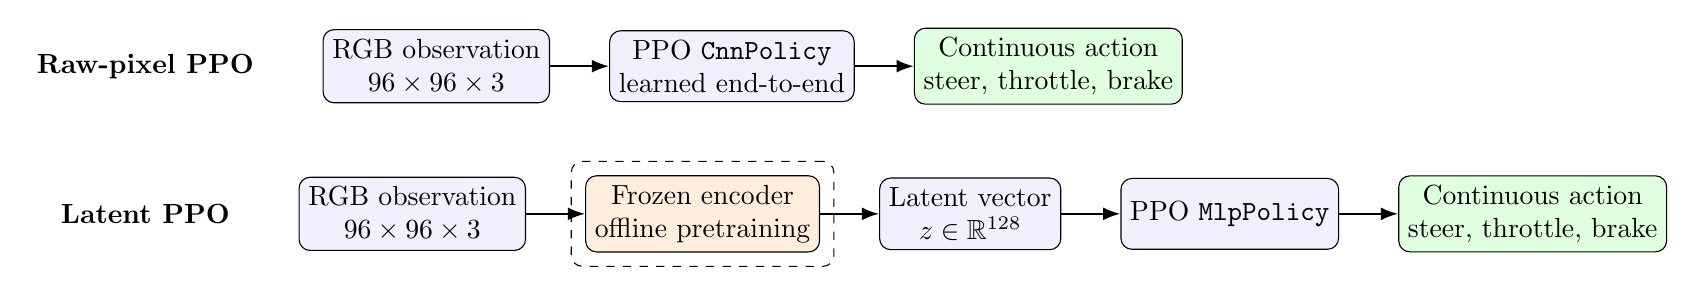
\begin{tikzpicture}[
  node distance=0.7cm and 0.75cm,
  block/.style={draw, rounded corners, align=center, minimum height=0.9cm,
    minimum width=2.15cm, fill=blue!6},
  frozen/.style={block, fill=orange!13},
  action/.style={block, fill=green!12},
  arrow/.style={-{Latex[length=2.2mm]}, thick},
  label/.style={font=\bfseries}
]
\node[label] (rawlabel) {Raw-pixel PPO};
\node[block, right=of rawlabel] (rawobs) {RGB observation\\$96\times96\times3$};
\node[block, right=of rawobs] (cnn) {PPO \texttt{CnnPolicy}\\learned end-to-end};
\node[action, right=of cnn] (rawact) {Continuous action\\steer, throttle, brake};

\node[label, below=1.35cm of rawlabel] (latentlabel) {Latent PPO};
\node[block, right=of latentlabel] (latobs) {RGB observation\\$96\times96\times3$};
\node[frozen, right=of latobs] (encoder) {Frozen encoder\\offline pretraining};
\node[block, right=of encoder] (latent) {Latent vector\\$z\in\mathbb{R}^{128}$};
\node[block, right=of latent] (mlp) {PPO \texttt{MlpPolicy}};
\node[action, right=of mlp] (latact) {Continuous action\\steer, throttle, brake};

\draw[arrow] (rawobs) -- (cnn);
\draw[arrow] (cnn) -- (rawact);
\draw[arrow] (latobs) -- (encoder);
\draw[arrow] (encoder) -- (latent);
\draw[arrow] (latent) -- (mlp);
\draw[arrow] (mlp) -- (latact);

\node[draw, dashed, rounded corners, fit=(encoder), inner sep=5pt,
  label={[font=\scriptsize]below:weights fixed during PPO}] {};
\end{tikzpicture}
}
\caption{Controlled comparison between the raw-pixel baseline and the proposed
latent-observation pipeline. Both agents interact with the same environment and
use PPO; only the visual representation and policy architecture differ.}
\label{fig:pipeline}
\end{figure*}

\subsection{Environment}

The environment is \texttt{CarRacing-v3}, a Box2D continuous-control task
\cite{gymnasium_carracing}. The observation is an RGB image with shape
$96\times96\times3$ and \texttt{uint8} values. The action is a three-dimensional
continuous vector for steering, throttle, and brake. Experiments use
\texttt{lap\_complete\_percent=0.95} and
\texttt{domain\_randomize=False}. The default observation includes the
simulator HUD at the bottom of the frame. Keeping it in both conditions preserves
comparability, although it is a methodological limitation.

\subsection{Raw-Pixel Baseline}

The baseline follows the upper path in Fig.~\ref{fig:pipeline}. Stable-Baselines3
\cite{stable_baselines3} transposes observations to channel-first format and
trains PPO with \texttt{CnnPolicy}. Its convolutional extractor, actor, and value
function are optimized jointly from PPO rollouts. No external representation
pretraining or image augmentation is used.

\subsection{Frame Dataset}

Frames were sampled during earlier PPO interaction using random intervals to
reduce temporal redundancy. Sampling was delayed after environment resets to
avoid over-representing nearly identical starting frames. The resulting local
dataset contains 18,293 PNG images. Images are loaded as RGB, converted to
\texttt{float32}, normalized from $[0,255]$ to $[0,1]$, and transposed to
$3\times96\times96$. A fixed random split assigns 90\% of frames to training and
10\% to validation.

\begin{table}[t]
\centering
\caption{Autoencoder dataset summary.}
\label{tab:dataset}
\begin{tabular}{lc}
\toprule
\textbf{Property} & \textbf{Value}\\
\midrule
Source & CarRacing policy interaction\\
Samples & 18,293 RGB frames\\
Input format & $96\times96\times3$, PNG\\
Training split & 90\%\\
Validation split & 10\%\\
Normalization & Pixel values in $[0,1]$\\
\bottomrule
\end{tabular}
\end{table}

\subsection{Convolutional Autoencoder}

The encoder applies four stride-two convolutions with channel dimensions
$3\rightarrow32\rightarrow64\rightarrow128\rightarrow256$. Spatial resolution
is reduced from $96$ to $6$, producing a $256\times6\times6$ feature map. A
linear layer maps the flattened 9,216 values to a 128-dimensional latent vector.
The decoder mirrors this structure with a linear layer and four transposed
convolutions. A sigmoid output matches normalized RGB values.

For input $x$ and reconstruction $\hat{x}$, training minimizes mean squared
error:

\begin{equation}
\mathcal{L}_{\mathrm{AE}} =
\frac{1}{CHW}\sum_{c,h,w}(x_{c,h,w}-\hat{x}_{c,h,w})^2.
\end{equation}

The model was trained with Adam, batch size 128, and learning rate $10^{-4}$ for
40 epochs in two consecutive 20-epoch sessions. Before the second session, the
model weights were retained while the Adam optimizer was reinitialized. The
final training and validation losses are 0.000581 and 0.000659, respectively.
The model has approximately 3.75 million parameters.

\begin{figure}[t]
\centering
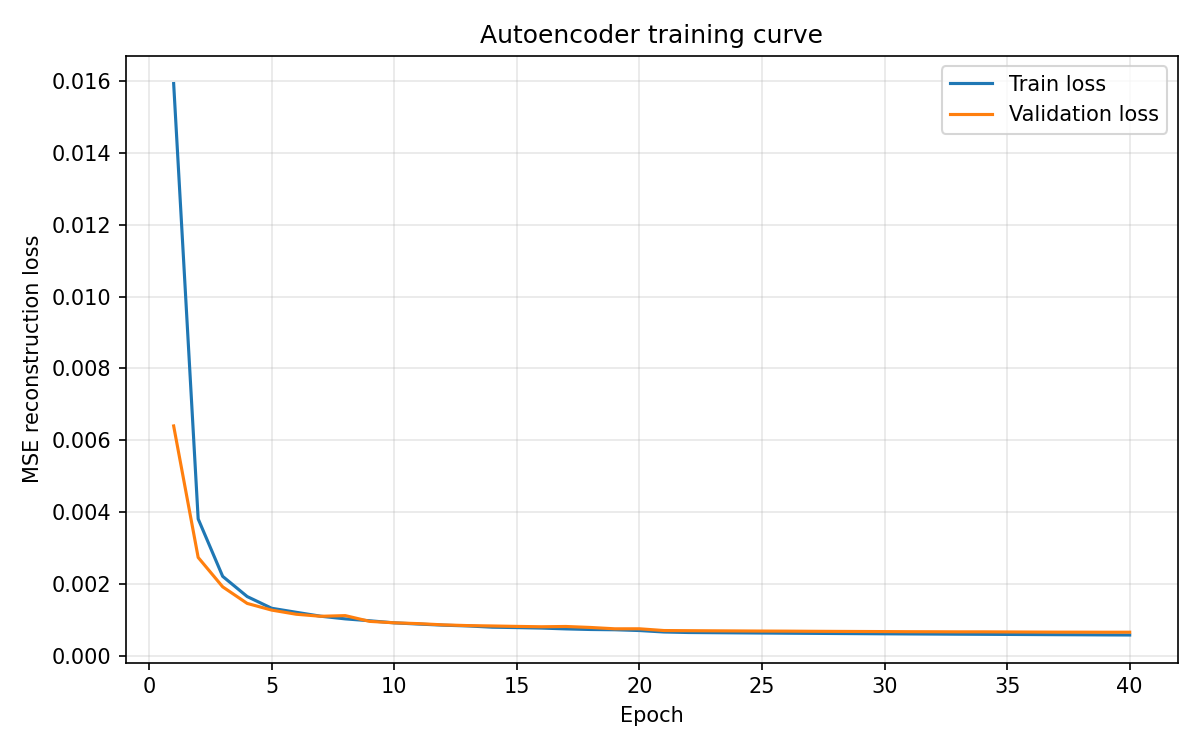
\includegraphics[width=\columnwidth]{figures/autoencoder_loss_curve.png}
\caption{Autoencoder training and validation MSE over 40 epochs.}
\label{fig:ae_loss}
\end{figure}

\begin{figure}[t]
\centering
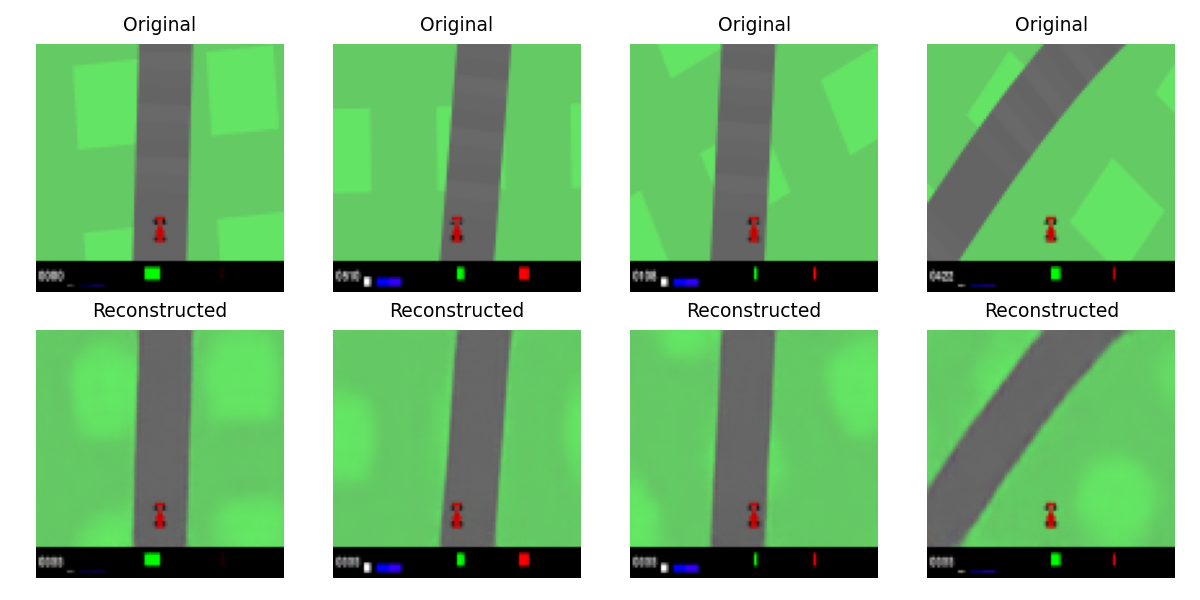
\includegraphics[width=\columnwidth]{figures/autoencoder_reconstructions_paper.png}
\caption{Original CarRacing observations (top) and autoencoder reconstructions
(bottom). Global road geometry and car position are retained, while boundaries
and textures are smoothed by the pixel-wise MSE objective.}
\label{fig:reconstructions}
\end{figure}

\subsection{Latent Observation Pipeline}

The lower path in Fig.~\ref{fig:pipeline} is implemented through a Gymnasium
observation wrapper. For each observation, the wrapper reproduces autoencoder
preprocessing, executes the encoder without gradient tracking, and returns a
128-dimensional \texttt{float32} vector. Encoder parameters are frozen and the
model remains in evaluation mode. PPO then uses \texttt{MlpPolicy}. Consequently,
the RL optimizer cannot adapt the visual representation to the control task.
This restriction is intentional because it isolates the effect of offline
reconstruction pretraining.

\begin{figure*}[t]
\centering
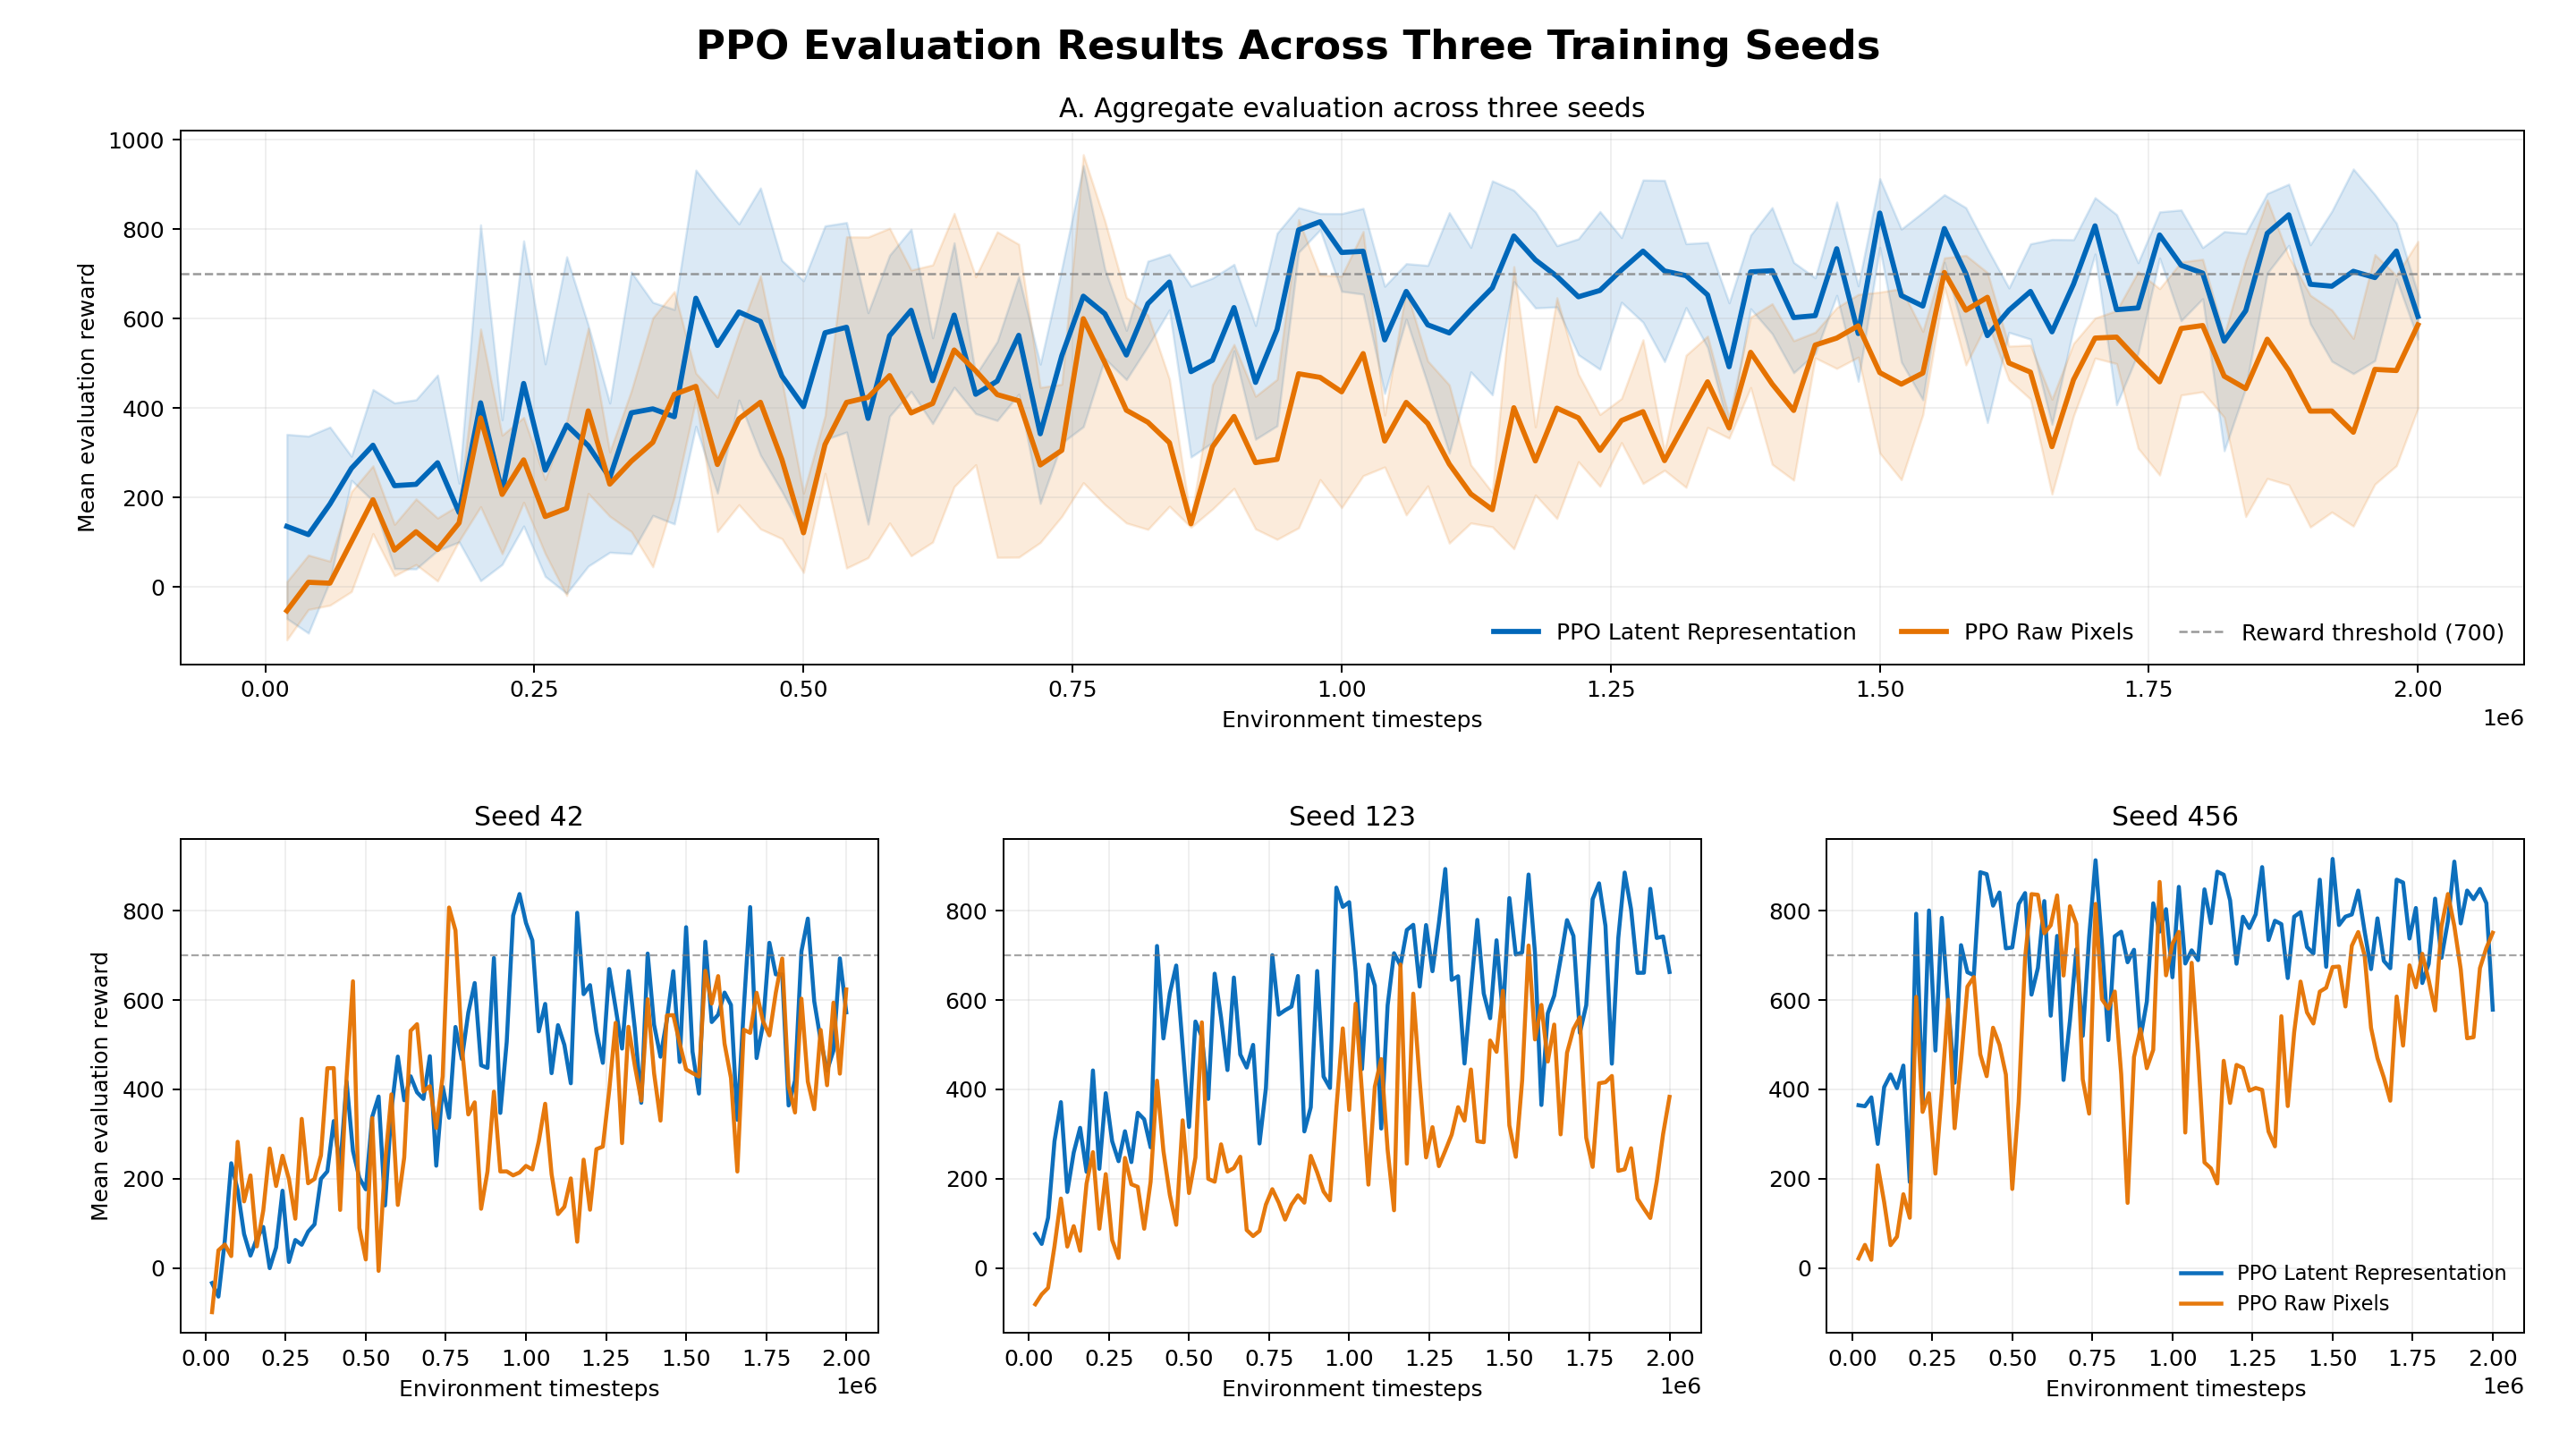
\includegraphics[width=0.98\textwidth]{figures/ppo_results_dashboard.png}
\caption{Deterministic PPO evaluation results. The upper panel shows the mean
reward across three training seeds, with shaded regions indicating one
between-seed standard deviation. The lower panels compare raw and latent PPO
within each matched seed. Each point averages five evaluation episodes.}
\label{fig:main_results}
\end{figure*}

\section{Experimental Setup}

\subsection{Software and Hardware}

The implementation uses Python 3.11, PyTorch, Gymnasium 1.2.3, and
Stable-Baselines3 2.8.0. Experiments run on an NVIDIA
GeForce RTX 3080 Ti and an AMD Ryzen 7 5800X CPU. Raw-pixel PPO uses CUDA,
whereas latent PPO and its frozen encoder use the CPU in the current
configuration.

\subsection{Controlled Multi-Seed Protocol}

The main benchmark consists of three independent training seeds,
$\{42,123,456\}$, for each method. Both methods use the same PPO learning rate,
interaction budget, number of parallel environments, and deterministic
evaluation protocol. Training and evaluation use distinct seeds. The evaluation
seed is fixed across methods so corresponding policies are tested on the same
procedurally generated tracks.

\begin{table}[t]
\centering
\caption{Main controlled PPO configuration.}
\label{tab:training}
\begin{tabular}{lc}
\toprule
\textbf{Parameter} & \textbf{Value}\\
\midrule
Algorithm & PPO\\
Training seeds & 42, 123, 456\\
Evaluation base seed & 10,000\\
Parallel environments & 2\\
Interaction budget & 2,000,000 steps\\
Learning rate & $10^{-4}$\\
Evaluation interval & 20,000 steps\\
Episodes per evaluation & 5\\
Raw policy & \texttt{CnnPolicy}\\
Latent policy & \texttt{MlpPolicy}\\
Latent dimension & 128\\
\bottomrule
\end{tabular}
\end{table}

The callback parameter is set to 10,000 calls. Because two vectorized
environments advance at each callback step, this corresponds to 20,000 aggregate
environment timesteps between evaluations. Each evaluation averages five
deterministic episodes. The best checkpoint is selected by evaluation reward,
and the final checkpoint is also retained.

\subsection{Metrics}

The following metrics are defined before observing the controlled benchmark:

\begin{itemize}
  \item best mean deterministic evaluation reward;
  \item timestep of the best evaluation;
  \item mean reward over the final five evaluations;
  \item normalized area under the evaluation learning curve (AUC);
  \item first timestep at which mean reward reaches 700;
  \item mean and standard deviation of scalar metrics across training seeds.
\end{itemize}

The final-window mean is preferred over a single last evaluation because
CarRacing returns are noisy and PPO learning is non-monotonic. Wall-clock time is
not a primary metric because the two policies use different devices and runs may
be scheduled at different times.

\subsection{Controlled Results}

Table~\ref{tab:main_results} reports the aggregate metrics across the three
training seeds. Latent PPO performs better on all four predefined aggregate
metrics. Its mean best evaluation reward increases from 798.1 to 882.4, while
the final-window mean increases from 459.2 to 685.1. The larger improvement in
final-window reward indicates that the latent policies maintain stronger
performance near the end of training rather than only producing an isolated
high-reward checkpoint.

\begin{table}[t]
\centering
\caption{Controlled results across three training seeds. Values are
mean $\pm$ standard deviation across seeds. For steps to reward 700, lower is
better.}
\label{tab:main_results}
\resizebox{\columnwidth}{!}{%
\begin{tabular}{lccc}
\toprule
\textbf{Metric} & \textbf{Raw PPO} & \textbf{Latent PPO} &
\textbf{Relative difference}\\
\midrule
Best evaluation reward & $798.1 \pm 71.7$ & $\mathbf{882.4 \pm 40.5}$ & $+10.6\%$\\
Final-window reward & $459.2 \pm 211.3$ & $\mathbf{685.1 \pm 127.4}$ & $+49.2\%$\\
Normalized AUC & $377.8 \pm 120.0$ & $\mathbf{567.5 \pm 134.5}$ & $+50.2\%$\\
Steps to reward 700 & $960\mathrm{k} \pm 529\mathrm{k}$ &
$\mathbf{520\mathrm{k} \pm 394\mathrm{k}}$ & $-45.8\%$\\
\bottomrule
\end{tabular}
}
\end{table}

Figure~\ref{fig:main_results} shows that the latent mean curve is higher through
most of training and crosses the reward-700 threshold earlier on average. The
matched-seed panels also expose substantial PPO variance. Latent PPO reaches the
threshold earlier for seeds 123 and 456, whereas raw PPO reaches it earlier for
seed 42. Nevertheless, latent PPO obtains higher best reward, final-window
reward, and normalized AUC in all three matched seeds.

\subsection{Critical Discussion}

The results support three cautious observations. First, a frozen
128-dimensional representation retains sufficient information for PPO to learn
effective driving behaviour despite compressing 27,648 pixel values. The
consistent improvements in AUC and final-window reward suggest that offline
visual pretraining simplified policy learning in this experimental setting.
Second, the benefit is not explained only by a fortunate checkpoint: latent PPO
achieves higher best reward, final-window reward, and normalized AUC for every
matched training seed.

Third, the frozen representation does not eliminate RL instability. The shaded
regions in Fig.~\ref{fig:main_results} remain wide, and threshold-crossing time
has large standard deviation for both methods. With only three seeds, the
experiment provides descriptive rather than strong inferential statistical
evidence. The results therefore support the latent pipeline within the tested
\texttt{CarRacing-v3} protocol, but they do not establish that reconstruction
pretraining is generally superior to end-to-end visual RL.

The comparison also changes the policy architecture from \texttt{CnnPolicy} to
\texttt{MlpPolicy}, because the observation spaces differ. This is intrinsic to
the research question but means the measured effect combines representation
pretraining, dimensionality reduction, and a smaller downstream policy input.
It should not be interpreted as an isolated ablation of encoder initialization.

\section{Limitations}

The experiment has several limitations. Three seeds improve reliability but
remain a small sample for a high-variance RL benchmark, and no significance test
is meaningful at this sample size. Evaluation averages only five episodes at
each checkpoint. The frame dataset was collected from policy interaction and
may under-represent rare recovery states. The HUD is included in all images, and
the autoencoder may allocate capacity to it. MSE encourages smooth
reconstructions and may suppress sharp road boundaries. The encoder is frozen,
preventing task-specific adaptation, and only one latent dimension and one main
learning rate are evaluated. Finally, conclusions are limited to
\texttt{CarRacing-v3} and may not generalize to other visual-control tasks.

\section{Conclusion}

This project implements a reproducible comparison between end-to-end raw-pixel
PPO and PPO trained from a frozen autoencoder representation in
\texttt{CarRacing-v3}. The pipeline includes policy-based frame collection, a
convolutional autoencoder, a latent observation wrapper, controlled PPO training,
deterministic evaluation, and multi-seed aggregation. Under the tested protocol,
latent PPO improves best reward by 10.6\%, final-window reward by 49.2\%, and
normalized AUC by 50.2\%, while reaching reward 700 with 45.8\% fewer timesteps
on average. The advantage appears across all three matched seeds for best
reward, final-window reward, and AUC, although both methods retain substantial
variance.

These findings indicate that a compact frozen representation can improve sample
efficiency and overall performance in this setting. They do not imply that low
reconstruction error guarantees generally useful control features. The main
contribution is therefore the complete reproducible pipeline and controlled
critical comparison, rather than a new RL algorithm.

Future work should evaluate cropped observations without the HUD, alternative
latent dimensions, visual augmentation, robustness to perturbations, and
task-aware encoder fine-tuning.

\section*{Acknowledgments}

The project uses the open-source Gymnasium, Stable-Baselines3, and PyTorch
ecosystems.

\bibliographystyle{plain}
\bibliography{references}

\end{document}
